\documentclass[20pt]{article}
\usepackage{graphicx}
\usepackage{titling}
\usepackage[utf8]{inputenc}
\usepackage[T1]{fontenc}
\usepackage{hyperref}
\usepackage{float} 
\usepackage[a4paper, margin=3cm]{geometry}
\usepackage[spanish]{babel}
\usepackage{xcolor}

\title{Benevolent Dictator For Life \\ \large Guido Van Rossum \\ \large (1956-hasta la fecha)}
\author{Benjamin Maldonado,
Catalina Medina y
Antonia León}
\date{Marzo 2025}

\begin{document}

\begin{titlepage}
    \centering
    {\huge {\textbf{Programanji} \\ \LARGE{Adivina Buen Adivinador} \\}}
    \vspace{4cm}

\begin{figure}[htp]
    \centering
    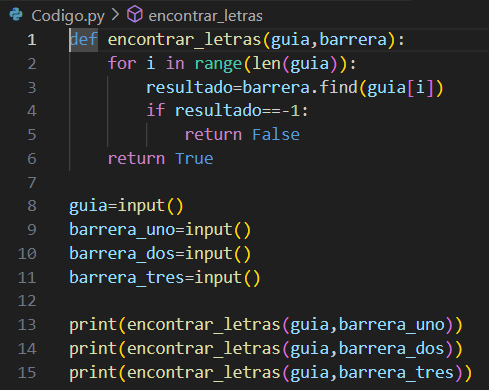
\includegraphics[width=15cm]{Codigo.png}
    \caption{Codigo}
    \label{fig:Codigo}
\end{figure}

\vfill
\centerline{\rule{15cm}{0.4mm}}
    {\large {Benjamin Maldonado}\par}
    {\large Fecha: \today\par}
\end{titlepage}
\newpage

\centerline{\underline{\LARGE{\textit{\textbf{\textcolor{red!40!black}{Creador}}}}}}
\addcontentsline{toc}{section}{Creador y proposito}
\vspace{0.5 cm} 

\section*{Descripción del código}

Este código, creado por mi, \textbf{Benjamin Maldonado}, como parte del set 5 de \textit{Clearn}, tiene como objetivo encontrar las letras de tres palabras específicas en una palabra guía. El código busca determinar si todas las letras de la palabra objetivo se encuentran presentes en la palabra guía, sin importar el orden en que aparecen.

\subsection*{Funcionalidad}

El código funciona de la siguiente manera:

\begin{itemize}
  \item Toma como entrada una palabra guía y una palabra barrera.
  \item Busca cada letra de la palabra barrera en la palabra guía.
  \item Si encuentra todas las letras de la palabra barera en la palabra guía, devuelve el valor booleano \texttt{True}.
  \item Si no encuentra todas las letras de la palabra barrera en la palabra guía, devuelve el valor booleano \texttt{False}.
\end{itemize}

\subsection*{Ejemplo}

Por ejemplo, si se utiliza la palabra guía \textit{``Grandilocuencia''} y la palabra barrera \textit{``Graaaandilocueenciaaa''}, el código buscaría las letras ``\texttt{G}, \texttt{r}, \texttt{a}, \texttt{n}, \texttt{d}, \texttt{i}, \texttt{l}, \texttt{o}, \texttt{c}, \texttt{u}, \texttt{e}, \texttt{n}, \texttt{c}, \texttt{i} y \texttt{a}'' en la palabra guía. Si encuentra todas estas letras, devolvería \texttt{True}; de lo contrario, devolvería \texttt{False}.

\subsection*{Utilidad}

Este código puede ser útil en diversas aplicaciones, como:

\begin{itemize}
  \item \textbf{Verificación de anagramas}: puede utilizarse para determinar si una palabra es un anagrama de otra.
  \item \textbf{Análisis de texto}: puede utilizarse para analizar la frecuencia de aparición de ciertas letras o palabras en un texto.
  \item \textbf{Juegos de palabras}: puede utilizarse en juegos de palabras que requieren encontrar palabras ocultas en otras palabras.
\end{itemize}

\subsection*{Conclusión}

En resumen, este código es una herramienta útil para encontrar las letras de una palabra objetivo en una palabra guía. Su funcionalidad es simple pero efectiva, y puede ser utilizado en diversas aplicaciones que requieren análisis de texto o verificación de anagramas.


\end{document}
